\section{Loss functions}

Since there are two ANN, two loss functions were obtained with the training. They are shown in the~\cref{fig:test_loss}.

\begin{figure}[!htb]
    \centering
    \caption[Loss Functions Behavior]{Loss Functions Behavior. The total number of epochs is 500 and was omitted because they were approximating a straight line.}
    %
    \begin{subfigure}{0.49\textwidth}
        \centering
        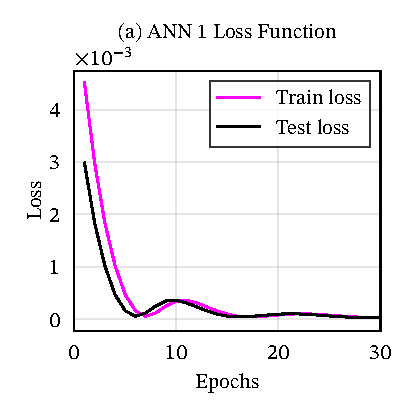
\includegraphics{figures/4results/uav/loss_function_nn1.pdf}
    \end{subfigure}
    \hfill
    \begin{subfigure}{0.49\textwidth}
        \centering
        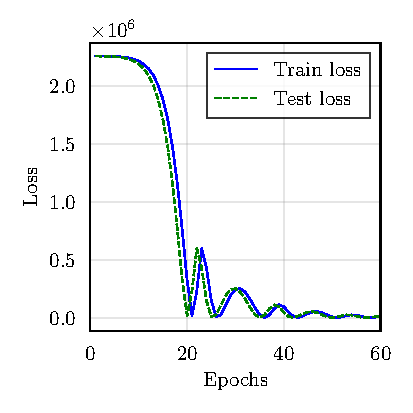
\includegraphics{figures/4results/uav/loss_function_nn2.pdf}
    \end{subfigure}

    \fonte{prepared by the author.}
    \label{fig:test_loss}
\end{figure}

The expected behavior of the loss function is its decay as the epochs increases.
\cref{fig:test_loss} shows the loss function decreasing along the epochs for both ANN and both for the train and test data.
The data used for training is relatively small (1000) and after splitting the data, for the training, indeed, the ANN only could see the pattern of 800 trajectories.
One of the strategies, therefore, was to use a high number of epochs, even though the loss function had already converged.
For acknowledgment, the convergence began with the first 10\% of the total number of epochs for both ANNs.
This way, it was necessary to verify if the ANN was not going to overfit the data. However, as the green curve shows, the test validation also converged, making it much more likely that no overfitting occurred.



\section{UAV Forces}

The normalized forces from neural network ANN 1 go through a comparison with the white box script within the corresponding state space. 
This analysis is crucial because it reveals the consistency of the model, aiming to show insights into the accuracy of ANN 1 predictions.
The results are presented in~\cref{fig:forces_normalized}.
The denormalized forces obtained by joining the results of both ANN are also presented in~\cref{fig:forces_denormalized}, with the same goal.

The ANN 1 is supposed to determine patterns for the UAV forces based on its state space.
To achieve a better recognition of these patterns, normalization was performed to prevent the scale of the values from affecting the ANN, since the input values have different units of measurement among themselves and also differ from the output values.

The recognized pattern will serve as the main basis for denormalization when the algorithm is applied. As can be seen in~\cref{fig:forces_normalized}, for \(U_2\) and \(U_4\), although the maximum and minimum local values do not match, the ANN could determine the pattern of the forces, following the raise and the fall of the real value.
After stabilization, that is, when the UAV stops increasing in the \(z(t)\) direction, both curves overlap.
For \(U_3\), it is noticed that after stabilization, the curves also overlap. However, before that, the decay pattern was recognized, but with some caveat.
At the global minimum value of the real output, the ANN could not follow the pattern as it should; in fact, it went in the opposite direction. This can affect directly in the UAV trajectory and compromise the flight.
For \(U_1\), on the other hand, the recognition was poor, and for the UAV takeoff, the ANN could not determine the force to keep the flight going.
After stabilization, although it improved compared to the beginning of the trajectory, the oscillations are high enough to compromise the flight.

\begin{figure}[!htb]
    \centering
    \caption[Normalized Forces from ANN 1]{Normalized Forces from ANN 1. Comparison is made from the results predicted from the neural network and the normalized preprocessing data, both for input and output data.}
    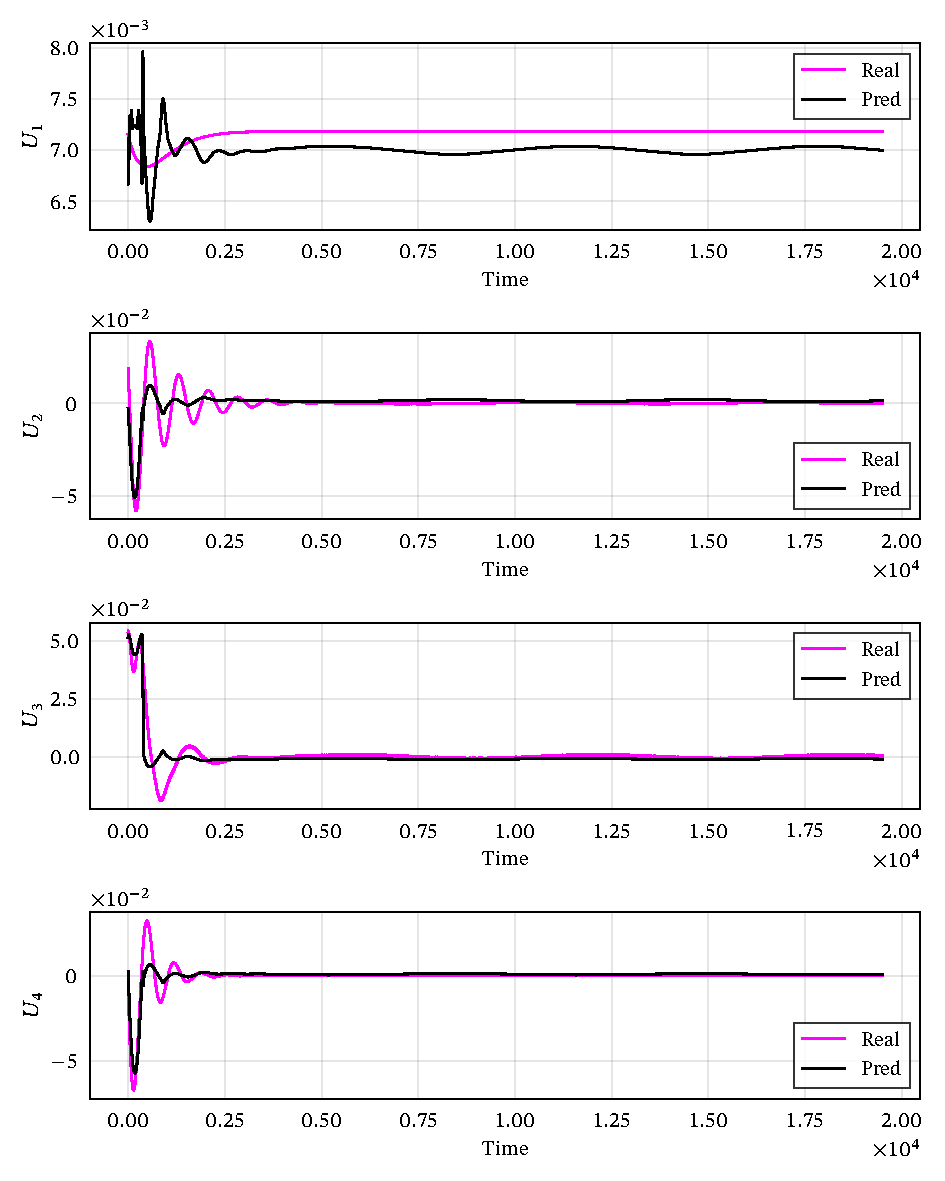
\includegraphics{figures/4results/uav/forces_normalized.pdf}

    \fonte{prepared by the author.}
    \label{fig:forces_normalized}
\end{figure}

As can be seen in~\cref{fig:forces_denormalized}, the curves are pratically identical to the normalized ones, but with different order of magnitude.
This shows that ANN 2 had great performance in recognizing the norm patterns, especially considering the stabilization region.
For \(U_2\), \(U_3\) and \(U_4\) the curves are overlapping, and the order of magnitude is very low, indicating good accuracy.
For \(U_1\), as happened with ANN 1, it did not perform as well, and the difference is bigger from the real value compared to the other ones. Yet, after stabilization, the ANN was precise, but not exact. 
If this pattern continues for all predicted forces, it can be adjusted with a factor to correct this.
Let \(\alpha\) be this \emph{correction factor}. 
If it is observed that the predicted values from the ANN consistently underestimate the original values by one unit, as occurred in \(U_1\), then it can be assumed \(\alpha = 1\).

\begin{figure}[!htb]
    \centering
    \caption[Denormalized Forces from ANN 1 and ANN 2 Combination]{Denormalized Forces from ANN 1 and ANN 2 Combination. Comparison is made from the results predicted from the combination of both neural network and the raw data got from the white box parametric model.}
    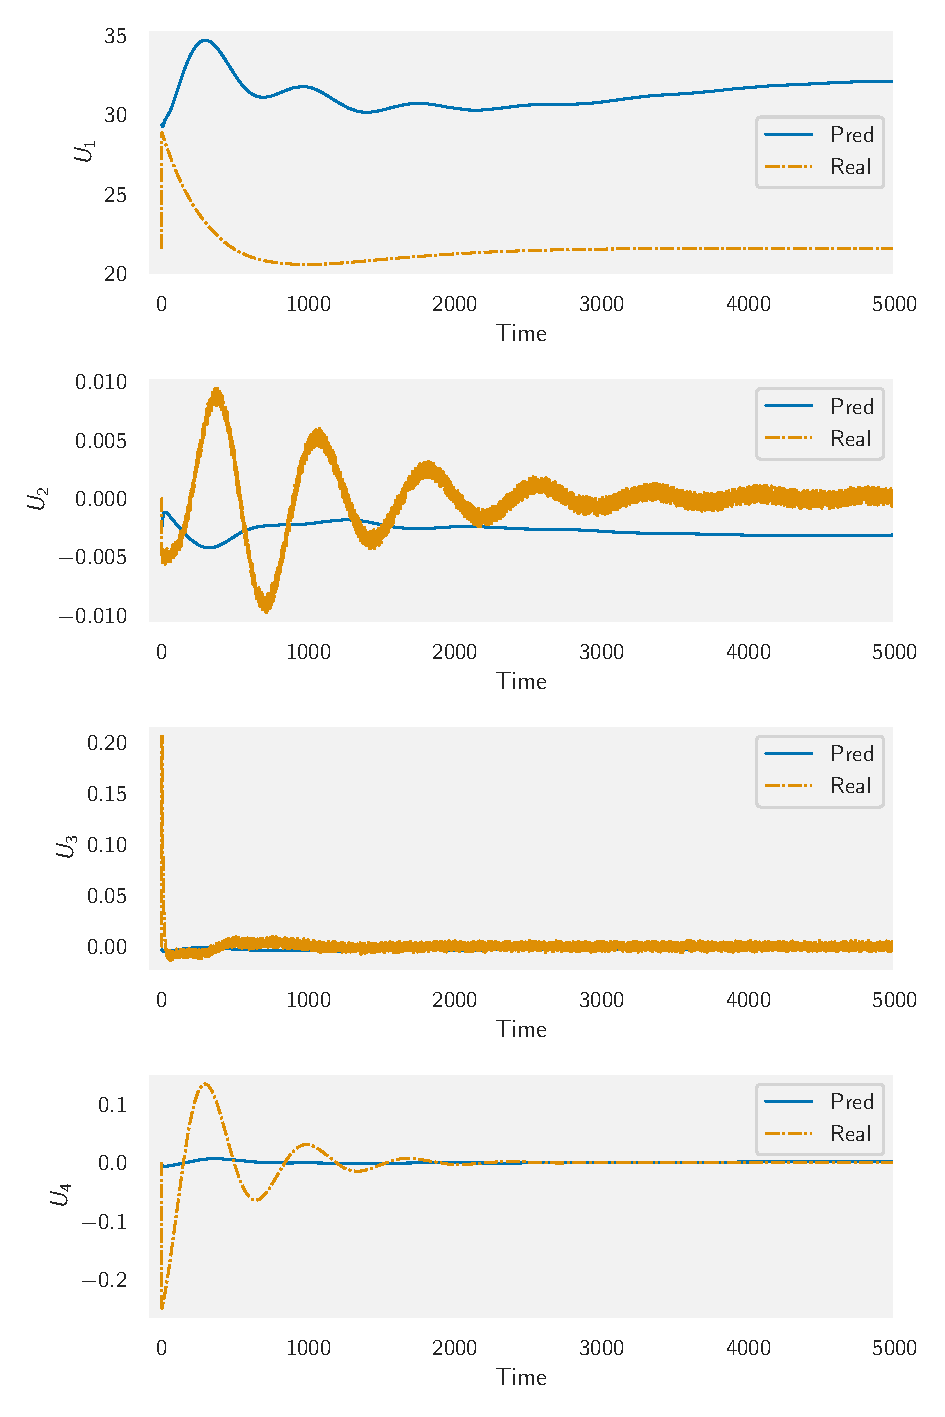
\includegraphics{figures/4results/uav/forces_denormalized.pdf}    

    \fonte{prepared by the author.}
    \label{fig:forces_denormalized}
\end{figure}

The main problem of the ANN is the quantity of the samples.
For a ANN, it is necessary a large amount of samples, at least hundreds of thousands of them. 
The data generation was limited by some factors: (i) computational resources, which were not sufficient to generate more than two thousand matrices with twenty thousand lines; (ii) the MATLAB version used, which could not generate files over 2 GB to export the files generated to the Python environment. These situations can be improved with powerful data processing and by using newer MATLAB versions.

This initial approach used a MLP, which is a  simple ANN architecture.
Although efficient for regression problems, the limited quantity of samples hindered its capability to determine the patterns more efficiently.
Therefore, exploring alternative ANNs architectures and approaches that can use less data and get more results is an alternative.
Since the methodology used is in the AI field, then machine learning techniques can also be a good approach, due to the data nature that is structured and well-defined matrices.

One alternative strategy is to split the trajectory and use different ANN for each part or to use different ANN to each force separately. 
This can reduce bias from the different trajectories or forces.
The takeoff pattern is very different of when the UAV reaches the desired altitude.
Therefore, splitting one ANN for takeoff and another for the already defined trajectory may be a good approach.


Finally, this is the initial attempt utilizing ANN. 
Therefore, it started with the simplest available method, achieving satisfactory results within this scenario. The objective is to begin with a straightforward approach and refine the methodology as necessary. Using pre-trained models for regression is also a feasible alternative, involving adjustments to a few layers and tweaking to this specific problem. As the sample size increases and the ANN becomes more complex, the predictions can become more accurate.







